%!TEX root = ED_Arvore.tex

\section{Balanceamento Estático DSW}
\begin{frame}[label=notas]
	Day/Stout/Warren: a árvore é transformada em um \emph{backbone} (árvore degenerada em lista) que é transformado em uma árvore balanceada
	\\\vfill\pause
	Não é aplicado a cada operação na árvore.
		\subitem{O custo é amortizado ao longo do uso.}
\end{frame}

\begin{frame}[label=notas]
	Rotação:
	\begin{itemize}
		\item altera a estrutura [local] da árvore binária
		\item não altera o ordenamento dentro da árvore binária
	\end{itemize}
	\vfill
	\begin{center}
		
\includegraphics[width=.9\textwidth]{Tree_rotation}
	\end{center}
\end{frame}

\begin{frame}[label=notas]
	Rotação a direita\\\vfill
	\huge
	\begin{columns}[T]
		\column{.5\textwidth}\centering
			\begin{tikzpicture}[->, auto]
				\node (a) {A}
					child[missing] {}
					child {node[red] (e) {E}
						child {node (c) {C}
							child {node (b) {B}}
							child {node (d) {D}}
						}
						child[missing] {}
					}
				;
				\node<2 | handout:0>[rotate_right, fit=(c) (e)] {};
				\draw<3>[dotted,blueUnB!50,->, line width=3pt] (a)..controls +(south east:1) and +(north:1) .. (c); \node[blueUnB!50] at (a.east) {\normalsize{dir}};
				\draw<4>[dotted,greenUnB!50,->, line width=3pt] (e)..controls +(south west:1) and +(north:1) .. (d);  \node[greenUnB!50] at (e.west) {\normalsize{esq}};
				\draw<5>[dotted,blueUnB!50,->, line width=3pt] (c)..controls +(south east:2) and +(north east:2) .. (e);  \node[blueUnB!50] at (c.east) {\normalsize{dir}};
			\end{tikzpicture}
		\column{.5\textwidth}\centering
			\begin{tikzpicture}[->]
				\node<5-> {A}
					child[missing] {}
					child {node {C}
						child {node {B}}
						child {node {E}
							child {node {D}}
							child[missing] {}
						}
					}
				;
			\end{tikzpicture}
	\end{columns}
\end{frame}

\begin{frame}[label=notas]
	Criando backbone de árvore rotacionando a direita:\\
	\begin{columns}[T]
		\column{.2\textwidth}\centering
			\begin{tikzpicture}[->]
				\Tree [ .\node (a) {A};
						\edge[white]; \node {};
						[ .\node (e) {E}; 
							[ .C [ .B ] [ .D ] ] 
							[ .G [ .F ] \edge[white]; \node {}; ] ] ]
				\uncover<2 | handout:0>{\node[thickcircle, orange, fit=(a)] {};}
				\uncover<3 | handout:0>{\node[thickcircle, orange, fit=(e)] {};}
				\uncover<4>{\node[rotate_right, fit=(e)] {};}
			\end{tikzpicture}
		\column{.25\textwidth}\centering
			\uncover<5->{
			\begin{tikzpicture}[->]
				\Tree [ .A
						\edge[white]; \node {};
						[ .\node (c) {C}; 
							[ .B ] 
							[ .E 
								[ .D ] 
								[ .G [ .F ] \edge[white]; \node {}; ] ] ] ]
				\uncover<6 | handout:0>{\node[thickcircle, orange, fit=(c)] {};}
				\uncover<7>{\node[rotate_right, fit=(c)] {};}
			\end{tikzpicture}
			}
		\column{.25\textwidth}\centering
			\uncover<8->{
			\begin{tikzpicture}[->]
				\Tree [ .A
						\edge[white]; \node {};
						[ .\node (b) {B}; \edge[white]; \node {};
							[ .\node (c) {C};  \edge[white]; \node {};
								[ .\node (e) {E};
									[ .D ] 
									[ .G [ .F ] \edge[white]; \node {}; ] ] ] ] ]
				\uncover<9 | handout:0>{\node[thickcircle, orange, fit=(b)] {};}
				\uncover<10 | handout:0>{\node[thickcircle, orange, fit=(c)] {};}
				\uncover<11 | handout:0>{\node[thickcircle, orange, fit=(e)] {};}
				\uncover<12>{\node[rotate_right, fit=(e)] {};}
			\end{tikzpicture}
			}
		\column{.15\textwidth}\centering
			\uncover<13->{
			\begin{tikzpicture}[->]
				\Tree [ .A [ .B  [ .C   [ .\node (d) {D}; 
									[ .\node (e) {E}; \edge[white]; \node {};
										[  .\node (g) {G};  [ .F ] \edge[white]; \node {}; ] ] ] ] ] ]
				\uncover<14 | handout:0>{\node[thickcircle, orange, fit=(d)] {};}
				\uncover<15 | handout:0>{\node[thickcircle, orange, fit=(e)] {};}
				\uncover<16 | handout:0>{\node[thickcircle, orange, fit=(g)] {};}
				\uncover<17>{\node[rotate_right, fit=(g)] {};}
			\end{tikzpicture}
			}
		\column{.1\textwidth}\centering
			\uncover<18->{
			\begin{tikzpicture}[->]
				\Tree [ .A	[ .B [ .C  [ .D [ .E [  .F  [ .G ] ] ] ] ] ] ]
			\end{tikzpicture}
			}
	\end{columns}
	\vspace{-2em}
	\uncover<19->{Complexidade?} \uncover<20->{$O(n)$}
\end{frame}

% \begin{frame}[label=notas]
%  	Criando backbone de árvore rotacionando a esquerda:
%  	\begin{columns}[T]
%  		\column{.2\textwidth}\centering
%  			\begin{tikzpicture}[->]
%  				\Tree [ .\node (a) {A};
%  						\edge[white]; \node {};
%  						[ .E	[ .C [ .B ] [ .D ] ] 
%  						    	[ .G [ .F ] \edge[white]; \node {}; ] ] ]
%  				\uncover<2>{\node[thickcircle, orange, fit=(a)] {};}
%  				\uncover<3>{\node[rotate_left, fit=(a)] {};}
%  			\end{tikzpicture}
%  		\column{.2\textwidth}\centering
%  			\uncover<4->{
%  			\begin{tikzpicture}[->]
%  				\Tree [.\node (e) {E}; 
%  						[ .A  \edge[white]; \node {};
%  							[ .C [ .B ] [ .D ] ]  ]
%  						[ .G [ .F ] \edge[white]; \node {}; ] ]
%  				\uncover<5>{\node[thickcircle, orange, fit=(e)] {};}
%  				\uncover<6>{\node[rotate_left, fit=(e)] {};}
%  			\end{tikzpicture}
%  			}
% %		\column{.2\textwidth}\centering
% %			\uncover<7->{
% %			\begin{tikzpicture}[->]
% %				\Tree [ .\node (g) {G};
% %						[ .\node (e) {E};
% %							[ .A  \edge[white]; \node {};
% %								[ .C [ .B ] [ .D ] ] ] 
% %							[ .F ] ] 
% %						\edge[white]; \node {}; ]
% %				\uncover<8>{\node[thickcircle, orange, fit=(g)] {};}
% %				\uncover<9>{\node[thickcircle, orange, fit=(e)] {};}
% %				\uncover<10>{\node[rotate_left, fit=(e)] {};}
% %			\end{tikzpicture}
% %			}
% %		\column{.2\textwidth}\centering\hrule
% %			\uncover<11->{
% %			\begin{tikzpicture}[->]
% %				\Tree [ .G [ .\node (f) {F};
% %							[ .\node (e) {E};
% %								[ .\node (a) {A};  \edge[white]; \node {};
% %									[ .C [ .B ] [ .D ] ] ]
% %								\edge[white]; \node {}; ] ] ]
% %				\uncover<12>{\node[thickcircle, orange, fit=(f)] {};}
% %				\uncover<13>{\node[thickcircle, orange, fit=(e)] {};}
% %				\uncover<14>{\node[thickcircle, orange, fit=(a)] {};}
% %				\uncover<15>{\node[rotate_left, fit=(a)] {};}
% %			\end{tikzpicture}
% %			}
%  		\column{.15\textwidth}\centering
%  			\uncover<7->{
%  				{\Huge \vfill ... \vfill}
% %			\begin{tikzpicture}[->]
% %				\Tree [ .G [ .F [ .E
% %							[ .\node (c) {C}; 
% %								[ .A \edge[white]; \node {}; [ .B ] ] 
% %								[ .D ] ]
% %							\edge[white]; \node {}; ] ] ]
% %				\uncover<17>{\node[thickcircle, orange, fit=(c)] {};}
% %				\uncover<18>{\node[rotate_left, fit=(c)] {};}
% %			\end{tikzpicture}
%  			}
%  		\column{.15\textwidth}\centering
%  			\uncover<7->{
%  			\begin{tikzpicture}[->, level distance=1cm]
%  				\Tree [ .G [ .F [ .E [ .\node (d) {D}; [  .\node (c) {C}; 
%  									[ .\node (a) {A}; \edge[white]; \node {}; [ .B ] ] ] ] ] ] ]
%  				%\uncover<8>{\node[thickcircle, orange, fit=(d)] {};}
%  				%\uncover<9>{\node[thickcircle, orange, fit=(c)] {};}
%  				%\uncover<10>{\node[thickcircle, orange, fit=(a)] {};}
%  				\node<7>[rotate_left, fit=(a)] {};
%  			\end{tikzpicture}
%  			}
%  		\column{.05\textwidth}\centering
%  			\uncover<8->{
%  			\begin{tikzpicture}[->, level distance=1cm]
%  				\Tree [ .G [ .F [ .E [ .D [ .C [ .B [ .A ] ] ] ] ] ] ]
%  			\end{tikzpicture}
%  			}
%  	\end{columns}
% \end{frame}

\begin{frame}[fragile,label=notas]
	\begin{center}\begin{minipage}{.85\textwidth}
		\begin{lstlisting}[morekeywords={balanceamento_dsw,em_backbone,altura,comprime,num_rotacoes}]
			comprime(raiz, num_rotacoes)
			    ptr := raiz
			    enquanto num_rotacoes > 0
			        rotacao_a_esquerda(ptr)
			        ptr :== ptr->dir
			        num_rotacoes := num_rotacoes - 1

			balanceamento_dsw(raiz)
			    em_backbone(raiz);
			    tam_backbone := altura(raiz) - 1
			    numero_de_rotacoes := tam_backbone/2
			    enquanto numero_de_rotacoes > 0
			        comprime(raiz, numero_de_rotacoes)
			        tam_backbone := tam_backbone - (numero_de_rotacoes + 1)
			        numero_de_rotacoes := tam_backbone/2
		\end{lstlisting}
		% \begin{lstlisting}[morekeywords={dsw_backbone, dsw_comprime}]
		%	void bt_balanceamento_dsw(bst_elemento_t **ptr_raiz) {
		%	  dsw_backbone(ptr_raiz);
		 	    
		%	  int tam_backbone = bt_altura(*ptr_raiz) - 1;
		%	  int numero_de_rotacoes = tam_backbone/2;
		%	  while(numero_de_rotacoes > 0) {
		%	    dsw_comprime(ptr_raiz, numero_de_rotacoes);
		%	    tam_backbone -= numero_de_rotacoes + 1;
		%	    numero_de_rotacoes = tam_backbone/2;
		%	  }
		%	}
		% \end{lstlisting}
	\end{minipage}\end{center}
	\subitem{Árvore balanceada \alert<4>{completa} teria altura $k$ e $2^k-1$ nós em cada nível}
\end{frame}

\begin{frame}[label=notas]
	\begin{columns}[T]
		\column{.4\textwidth}\centering
			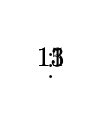
\begin{tikzpicture}[->, level distance=1cm]
				\Tree [ .\node (15) {15};
						[ .14
							[ .\node (13) {13};
								[ .12
									[ .\node (11) {11};
										[ .10
											[ .\node {$\vdots$}; ]
												%\edge[dotted]; \node {}; %[ .\node (8) {8};	]
												%\edge[white]; \node {};
											\edge[white]; \node {};
										] \edge[white]; \node {};
									] \edge[white]; \node {};
								] \edge[white]; \node {};
							] \edge[white]; \node {};
						] \edge[white]; \node {};
					  ]
				\uncover<3->{\rotateright{11,13,15}}
			\end{tikzpicture}
			\\\pause
			%$tam\_backbone$ = 14,\hfill\\$numero\_de\_rotacoes$ = 7
		\column{.6\textwidth}\centering
			\uncover<4->{
			
\begin{tikzpicture}[->, level distance=1cm]
				\Tree [ .\node (14) {14};
						[ .12
							[ .\node (10) {10};
								[ .8
									[ .\node (6) {6};
									         	[ .4
									         		[ .2 [ .1 ]	[ .3 ]  ]
									         		[ .5 ]
									         	] [ .7 ]
									]  [ .9 ]	
								] [ .11 ]
							] [ .13 ]
						] [ .15 ]
					  ]
				\uncover<4->{\rotateright{6,10,14}}
			\end{tikzpicture}}
	\end{columns}
\end{frame}

\begin{frame}[label=notas]
	\begin{columns}[T]
		\column{.5\textwidth}\centering
			\begin{tikzpicture}[->]
				\Tree [ .\node (12) {12};
						[ .8
							[ .4  [ .2 [ .1 ] [ .3 ] ] 
								  [ .6 [ .5 ] [ .7 ] ] ]
							[ .10 [ .9 ] 
								  [ .11 ] ] ]
						[ .14 [ .13 ] [ .15 ] ]  ]
				\node[rotate_right, fit=(12)] {};
			\end{tikzpicture}
			% \\$tam\_backbone$ = 2,\hfill\\$numero\_de\_rotacoes$ = 1
		\pause
		\column{.5\textwidth}\centering
			\begin{tikzpicture}[->]
				\Tree [ .8
						[ .4
							[ .2 [ .1 ]	[ .3 ] ]
							[ .6 [ .5 ]	[ .7 ] ] ]
						[ .12
							[ .10 [ .9 ]	[ .11 ] ]
							[ .14 [ .13 ] [ .15 ] ] ] ]
			\end{tikzpicture}
	\end{columns}
\end{frame}

\begin{frame}[label=notas]
	Exercícios:
	\begin{enumerate}[<+->]
		\item Árvore com 9 nós: backbone a esquerda
		\item Árvore com 12 nós: backbone a direita
	\end{enumerate}
	\begin{columns}[T]
		\column{.45\textwidth}\centering
			\uncover<2->{
			\begin{tikzpicture}[->, level distance=1cm]
				\Tree [ .4
						[ .2 [ .1 ]	[ .3 ] ]
						[ .6 [ .5 ]	[ .8 [ .7 ] [ .9 ] ] ] ]
			\end{tikzpicture}}
		\column{.45\textwidth}\centering
			\uncover<3->{\begin{tikzpicture}[->, level distance=1cm]
				\Tree [ .8
						[ .4 [ .2 [ .1 ] [ .3 ] ]	[ .6 [ .5 ] [ .7 ] ] ]
						[ .11 [ .10  [ .9 ] \edge[white]; \node {}; ] [ .12 ] ] ]
			\end{tikzpicture}}
	\end{columns}
\end{frame}